\section*{}
\begin{frame}
\frametitle{\secname}
\begin{figure}[!ht]
	\centering
	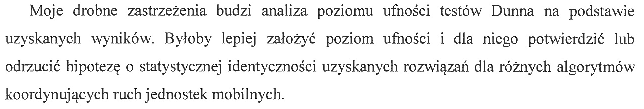
\includegraphics[page=1, width=0.9\textwidth]{img/ReviewZubert2.pdf}	
\end{figure}
\end{frame}

\section*{}
\begin{frame}
\frametitle{\secname}

Rzeczywiście, proponowana przez Pana Profesora procedura jest standardowo stosowana przy testowaniu hipotez statystycznych i taką drogą niewątpliwie powinienem był postępować. Przekroczenie często przyjmowanej  wartości $\alpha=0.05$ jako prawdopodobieństwo, poniżej którego spełniona jest hipoteza zerowa wystąpiło w teście tylko w wybranych przypadkach, dlatego też zakładając potencjalne przeredagowanie treści, jestem przekonany że doszedłbym do podobnych wniosków, pomimo, jak Pan Profesor zauważył, zastosowania testu w niekonwencjonalny sposób, czyli wykryłbym identyczność rozkładów  następujących obserwacji (szczegółowe zestawienie przesłane w wersji elektronicznej) przy jednoczesnym potwierdzeniu istotności różnicy rozkładów opisujących pozostałe obserwacje. Oczywiście zastosuje się do uwagi Pana Profesora w kolejnych pracach, podczas analizy statystycznej wyników przeprowadzonych eksperymentów.

\note{
Rzeczywiście, proponowana przez Pana Profesora procedura jest standardowo stosowana przy testowaniu hipotez statystycznych i taką drogą niewątpliwie powinienem był postępować. Przekroczenie często przyjmowanej  wartości $\alpha=0.05$ jako prawdopodobieństwo, poniżej którego spełniona jest hipoteza zerowa wystąpiło w teście tylko w wybranych przypadkach, dlatego też zakładając potencjalne przeredagowanie treści, jestem przekonany że doszedłbym do podobnych wniosków, pomimo, jak Pan Profesor zauważył, zastosowania testu w niekonwencjonalny sposób, czyli wykryłbym identyczność rozkładów następujących obserwacji:

\begin{itemize}
	\item Eksperymenty symulacyjne:
	\subitem \textit{otwarta przestrzeń} ustawienie: \textit{4-6} obserwacja (R -- R+): $4,985193 \cdot 10^{-1}$; (rozdział \ref{Podsumowanie_eksperymenty_symulacyjne}), 	
	
	\subitem \textit{otwarta przestrzeń okrąg} ustawienie: \textit{dwanaście robotów}, obserwacja (RVO -- R+): $3,36788 \cdot 10^{-1}$; (rozdział \ref{Wyniki_Otwarta_przestrzen_prostopadle_Ustawienie w okrąg}),
	
	\subitem \textit{przejście przez drzwi} ustawienia: \textit{1-H1} obserwacja (R -- PF): $0,5$; (rozdział \ref{Podsumowanie_eksperymenty_symulacyjne}),
	
	\subitem \textit{przejście przez drzwi} ustawienia: \textit{H1-4} obserwacja (R+ -- PF+): $4,43920 \cdot 10^{-1}$; (rozdział \ref{Wyniki_Przejscie_przez_drzwi}),
	
	\subitem \textit{przejście przez drzwi} ustawienie: \textit{H9-8} obserwacja (R+ -- PF+): $8,60042 \cdot 10^{-2}$; (rozdział \ref{Wyniki_Przejscie_przez_drzwi}),
	
	\subitem \textit{Skrzyżowanie typu 8} ustawienie: \textit{cztery roboty} obserwacja (R -- R+): $3,035915 \cdot 10^{-1}$; (rozdział \ref{Podsumowanie_eksperymenty_symulacyjne}), 
	
	
	\item Eksperymenty z wykorzystanie rzeczywistych robotach:
	
	\subitem \textit{otwarta przestrzeń} ustawienie: \textit{1-2} obserwacja (R -- R+): $2,435655 \cdot 10^{-1}$; (rozdział \ref{Podsumowanie eksperymentów z wykorzystaniem rzeczywistych robotów}), 
	
	\subitem \textit{otwarta przestrzeń} ustawienie: \textit{skos [cztery roboty zadanie 2]} obserwacja (RVO -- R+): $4,363 \cdot 10^{-1}$; (rozdział \ref{Podsumowanie eksperymentów z wykorzystaniem rzeczywistych robotów}), 	
	
	\subitem \textit{przejście przez drzw} ustawienie: \textit{1-H1} obserwacja (PF -- PF+): $4,680237 \cdot 10^{-1}$; (rozdział \ref{Podsumowanie eksperymentów z wykorzystaniem rzeczywistych robotów}).	
\end{itemize}

przy jednoczesnym potwierdzeniu istotności różnicy rozkładów opisujących pozostałe obserwacje.
Oczywiście zastosuje się do uwagi Pana Profesora w kolejnych pracach, podczas analizy statystycznej wyników przeprowadzonych eksperymentów. 

}
\end{frame}


\section*{}
\begin{frame}
\frametitle{\secname}
\begin{figure}[!ht]
	\centering
	\includegraphics[page=4, width=0.8\textwidth]{img/ReviewZubert.pdf}	
\end{figure}
\end{frame}

\section*{}
\begin{frame}
\frametitle{\secname}
\normalsize

W symulacji roboty są reprezentowane przez wątki uruchamiane niezależnie i nie synchronizowane (4 roboty, 4 wątki). Każdy z wątków pobiera informacje ze wspólnego wątku zwanego \textit{serwerem lokalizacji}, który w oparciu o wyznaczone przez wątek robota sterowanie oblicza jego nową pozycję, aby następnie rozesłać informacje do wszystkich pozostałych wątków. Pozbawiając synchronizacji poszczególne wątki można było, chociaż w niewielkim stopniu, odwzorować działanie wątków do działania rzeczywistych robotów. Wątki odświeżają lokalizację robotów co ok. 200 ms, a następnie przeliczane jest nowe sterowanie według jednego z~algorytmów koordynacji (R, R+, PF, PF+, PR).
\newline
\newline
W eksperymentach na rzeczywistych robotach proces uruchamiany był na robocie, który wykonywał stosowne obliczenia związane z algorytmem koordynacji oraz sterowaniem kołami robota. Pozycja robota w tym przypadku dostarczana była z zewnętrznego systemu przez \textit{serwer lokalizacji} (system z kamerą oparty na markerach Aruco). W eksperymentach wykorzystujących rzeczywiste roboty mobilne krok czasowy jest bardzo ciężki do oszacowania z uwagi na wywłaszczenia systemu operacyjnego działającego na robocie czy czas potrzebny na odbiór i przetworzenie wiadomości z danymi o lokalizacji dostarczanymi z \textit{serwera lokalizacji}. W zaistniałej sytuacji pominięto w pracy krok czasowy jaki robot potrzebuje do wykonania pojedynczego cyklu (pobranie lokalizacji,  wyznaczenie trajektorii, przemieszczenie się). 


\note{
W symulacji roboty są reprezentowane przez wątki uruchamiane niezależnie i nie synchronizowane (4 roboty, 4 wątki). Każdy z wątków pobiera informacje ze wspólnego wątku zwanego \textit{serwerem lokalizacji}, który w oparciu o wyznaczone przez wątek robota sterowanie oblicza jego nową pozycję, aby następnie rozesłać informacje do wszystkich pozostałych wątków. Pozbawiając synchronizacji poszczególne wątki można było, chociaż w niewielkim stopniu, odwzorować działanie wątków do działania rzeczywistych robotów. Założono, iż procedury obliczeń związanych ze zlokalizowaniem robotów (obliczenia lokalizacji) oraz obliczenia związane z algorytmami będą trwały ok. 200 ms i~stąd przyjęto tę wartość kroku czasowego symulacji. Wątki odświeżają lokalizację robotów co ok. 200 ms, a następnie przeliczane jest nowe sterowanie według jednego z~algorytmów koordynacji (R, R+, PF, PF+, PR).

W eksperymentach na rzeczywistych robotach proces uruchamiany był na robocie, który wykonywał stosowne obliczenia związane z algorytmem koordynacji oraz sterowaniem kołami robota. Pozycja robota w tym przypadku dostarczana była z zewnętrznego systemu przez \textit{serwer lokalizacji} (system z kamerą oparty na markerach Aruco). W eksperymentach wykorzystujących rzeczywiste roboty mobilne krok czasowy jest bardzo ciężki do oszacowania z uwagi na wywłaszczenia systemu operacyjnego działającego na robocie czy czas potrzebny na odbiór i przetworzenie wiadomości z danymi o lokalizacji dostarczanymi z \textit{serwera lokalizacji}. W zaistniałej sytuacji pominięto w pracy krok czasowy jaki robot potrzebuje do wykonania pojedynczego cyklu (pobranie lokalizacji,  wyznaczenie trajektorii, przemieszczenie się). 


}
\end{frame}



\section*{}
\begin{frame}
\frametitle{\secname}
\begin{figure}[!ht]
	\centering
	\includegraphics[page=3, width=0.9\textwidth]{img/ReviewZubert2.pdf}	
\end{figure}
\end{frame}

\section*{}
\begin{frame}
\frametitle{\secname}
Istotnie ta kwestia powinna być w pracy lepiej doprecyzowana, iż w każdej chwili czasowej roboty posiadają swoje cele cząstkowe zaś kierunek ruchu rozpatrywany jest w bieżącej chwili czasowej dla lokalizacji robotów. Dziękuję za zwrócenie uwagi na wspomnianą niejednoznaczność, którą można było różnie interpretować. 
\end{frame}

\section*{}
\begin{frame}
\frametitle{\secname}
\begin{figure}[!ht]
\centering
\includegraphics[page=4, width=0.9\textwidth]{img/ReviewZubert2.pdf}	
\end{figure}
\end{frame}

\section*{}
\begin{frame}
\frametitle{\secname}
Bardzo dziękuję za tę sugestię. Z pewnością zgrabniej byłoby zmienić czy to szyk zdania lub rozwinąć szerzej wypowiedź tak, aby była bardziej przystępna oraz nie wzbudzała dyskomfortu w czytającym pracę.
\end{frame}

\section*{}
\begin{frame}
\frametitle{\secname}
\begin{figure}[!ht]
\centering
\includegraphics[page=5, width=0.9\textwidth]{img/ReviewZubert2.pdf}	
\end{figure}
\end{frame}

\section*{}
\begin{frame}
\frametitle{\secname}
Tak, oczywiście zgadzam się z Pana Profesora opinią, iż należało na wstępie określić zbiorczo, które ze współczynników należą do zbioru liczb rzeczywistych, a które przyjmują wartości dyskretne. Tym samym, można było unikać dodatkowych wstawek w tekście między innymi takich jak ,,pojedyncza liczba rzeczywista'' itp.
\end{frame}

\section*{}
\begin{frame}
\frametitle{\secname}
\begin{figure}[!ht]
\centering
\includegraphics[page=6, width=0.9\textwidth]{img/ReviewZubert2.pdf}	
\end{figure}
\end{frame}

\section*{}
\begin{frame}
\frametitle{\secname}
Bardzo dziękuję za to spostrzeżenie. Oczywiście jest to niedopatrzenie związane z~edytowaniem tekstu. W przyszłych pracach postaram się nie dopuścić do tego typu przeoczeń związanych z formatowaniem tekstu.
\end{frame}

\section*{}
\begin{frame}
\frametitle{\secname}
\begin{figure}[!ht]
\centering
\includegraphics[page=7, width=0.9\textwidth]{img/ReviewZubert2.pdf}	
\end{figure}
\end{frame}

\section*{}
\begin{frame}
\frametitle{\secname}
Bardzo dziękuję za tę uwagę. Istotnie w pracy zbyt często użyto słowa ,,stworzyć'', które można było częściej substytuować, przykładowo słowem ,,utworzyć'' czy ,,opracować''. W kolejnych pracach postaram się używać synonimów  tego słowa i nie nadużywać go zbyt często w ramach akapitów, sąsiadujących stron tekstu oraz całych rozdziałów.
\end{frame}